\documentclass{l4proj}

%
% put any additional packages here
%

\begin{document}

%==============================================================================
%% METADATA
\title{Level 4 Project: Particle-Based Video Prediction}
\author{Linh Giang Tran}
\date{February 13, 2023}
\maketitle

%==============================================================================
%% ABSTRACT
\begin{abstract}
    Every abstract follows a similar pattern. Motivate; set aims; describe work; explain results.
    \vskip 0.5em
    ``XYZ is bad. This project investigated ABC to determine if it was better. 
    ABC used XXX and YYY to implement ZZZ. This is particularly interesting as XXX and YYY have
    never been used together. It was found that  
    ABC was 20\% better than XYZ, though it caused rabies in half of subjects.''
\end{abstract}

%==============================================================================

% EDUCATION REUSE CONSENT FORM
% If you consent to your project being shown to future students for educational purposes
% then insert your name and the date below to  sign the education use form that appears in the front of the document. 
% You must explicitly give consent if you wish to do so.
% If you sign, your project may be included in the Hall of Fame if it scores particularly highly.
%
% Please note that you are under no obligation to sign 
% this declaration, but doing so would help future students.
%
%\def\consentname {Linh Giang Tran} % your full name
%\def\consentdate {28 February 2023} % the date you agree
%
\educationalconsent


%==============================================================================
\tableofcontents

%==============================================================================
%% Notes on formatting
%==============================================================================
%
% Do not alter the bibliography style.
%
% The first Chapter should then be on page 1. You are allowed 40 pages for a 40 credit project and 30 pages for a 20 credit report. This includes everything numbered in Arabic numerals (excluding front matter) up to but excluding the appendices and bibliography.
%
% You must not alter text size (it is currently 10pt) or alter margins or spacing.
%
%==================================================================================================================================
\chapter{Introduction}

\pagenumbering{arabic} % Reset page numbering. Don't remove this!

\section{Motivation}
Thanks to increased computational power and high volume of available data, notable progressions have been made in various deep learning fields. This has also sparked interest in employing end-to-end neural networks for video prediction which is of high relevance to numerous computer vision applications. By offering a glimpse into the future, next-frame prediction has the capability to improve environment understanding and decision-making in complex artificial intelligence systems, such as autonomous vehicles or robotics.

Traditional video prediction models generate the future frames by directly outputting the pixel RGB intensities of the target frame. While this is sufficient for some applications, direct pixel synthesis often produces blurry predictions as they fail to to robustly learn spatial and temporal dependencies in the frame. To elevate this issue, researchers experimented with incorporating higher level frame representations into video prediction models. For example, semantic segmentation or motion flow based models were able to report longer-term and more accurate predictions \citep{DBLP:journals/pami/OpreaMGCORA22}.

Unfortunately, obtaining a vast dataset of accurate trajectories in image sequences requires either  significant human labour or highly effective motion estimation methods. Although these methods have achieved noteworthy success, they are still susceptible to occlusions or significant appearance changes of tracked objects. Moreover, they do not account for pixel-level tracking across multiple frames.

In July 2022, \citeauthor{DBLP:journals/corr/abs-2204-04153} introduced a new 'particle video' approach called Persistent Independent Particles (PIPs), which demonstrated remarkable success by outperforming existing state-of-the-art models for motion estimation. This approach proved highly effective in handling occlusions across multiple frames. In light of this success, one might wonder whether it is feasible to leverage data generated by PIPs for future frame prediction.

\section{Aims and Objectives}
This project aims to investigate the effectiveness of an end-to-end neural network in predicting the next frame in a video sequence, using a dataset generated by Persistent Independent Particles (PIPs) approach. 

To methodically examine the problem, following objectives were identified:
\begin{itemize}
    \item Describe current state of future prediction research, main approaches and limitations (Section \ref{backgound})
    \item Create a dataset using PIPs ( Section \ref{implementation})
    \item Design and implement a deep learning model which will take a sequence of frames as input and output a point cloud prediction representing the coordinates of tracked pixels in the future frame (Section \ref{design} and \ref{implementation}) 
    \item Reconstruct frames using the model’s predictions (Section \ref{implementation})
    \item Evaluate the performance of the implemented neural network (Section \ref{evaluation})
\end{itemize}

%==================================================================================================================================
\chapter{Background} \label{backgound}
\section{Video Prediction}

The task of video prediction can be simply defined. Given a sequence of consecutive video frames $X_1, X_2, \dots, X_n$, the aim is to predict the future frames $X_{n+1}, X_{n+2}, \dots, X_{n+t}$ where n is number of input frames and t is the number of output frames to be predicted. For example, consider an image of a person riding a motorcycle (see Figure \ref{fig:motorbike}), it is likely that next frames will consist of the motorcycle moving across the frame to the left. This is a very simple task for humans as we have the ability to apply real-world experience to infer what might happen next.

On the contrary, this is extremely challenging for deep learning models because they have to be trained on large amount of high quality data to acquire the same level of prior knowledge that humans have. Moreover, the model may struggle to make good predictions due to inherent variability of possible outcomes in natural phenomena and complex interplay of multiple factors, such as appearance and position of various objects, illumination and layout of the scene or view-point and motion of the camera.

\begin{figure}
    \centering
    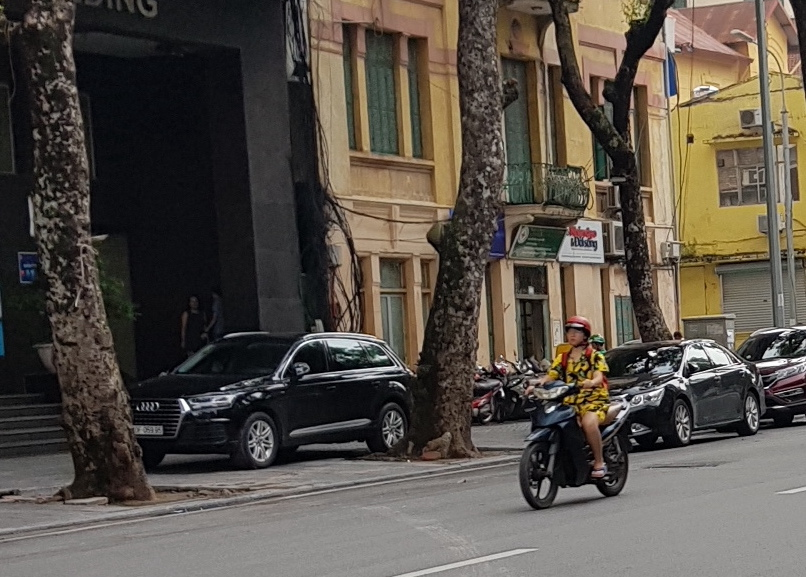
\includegraphics[width=0.6\linewidth]{images/motorbike.JPG}    
    \caption{\textbf{A video frame of a person riding a motorcycle.} While humans can easily infer the motorcycle will continue moving across the frame to the left in the future frames, this is a very challenging task for deep learning models.}
    \label{fig:motorbike} 
\end{figure}

\subsection{Single Image \& Multi-Frame Input}
Depending on the number of input frames, video prediction models can be divided into two strands: a single image or sequence of images input.

In singe image video prediction, the model predicts the next frame in a video sequence based on one static input image, without any additional context. Because a single image provides only a snapshot of a particular moment in time, it has significant limitations in representing unpredictability of systems. To address these limitations, researchers have developed a variety of techniques for incorporating stochasticity in single image input models. One common approach is to use generative models, such as variational autoencoders (VAEs) or generative adversarial networks (GANs) to learn a probabilistic representation of the data \citep{DBLP:journals/corr/XueWBF16, DBLP:journals/corr/WalkerDGH16, DBLP:journals/corr/abs-1802-07687, DBLP:journals/corr/abs-1804-01523}. This allows the model to capture the full range of variability in the data, and to generate new samples that are consistent with the underlying distribution of the data.

Still, many current prediction models are designed under the assumption of a deterministic environment \citep{DBLP:journals/corr/VondrickPT15, DBLP:journals/corr/LotterKC16, DBLP:journals/corr/RanzatoSBMCC14, DBLP:journals/corr/SrivastavaMS15}. While the future is inherently multi-modal, there are some situations where a deterministic prediction may be sufficient. For example, in many cases, the movement of a car can be largely deterministic, with only a small degree of uncertainty. In such deterministic situations, leveraging the time dimension of a multi-frame input can encourage the model to explicitly reason about object motion cues present in video sequences and hence help reduce the degree of uncertainty in predictions. Although multi-frame input model is able to generate more accurate predictions, it requires more computational resources than single image input models and therefore may not be suitable for real-time applications.

\subsection{Direct Pixel Predictions}
To utilise the large amount of available unlabeled videos, early video prediction models relied on directly predicting raw pixel RGB values \citep{DBLP:journals/corr/KalchbrennerOSD16, DBLP:journals/corr/SrivastavaMS15, DBLP:journals/corr/RanzatoSBMCC14}. Since any next frame serves as a label to previous frames in a video sequence, no additional human supervision for training is required. Therefore, it is reasonable to directly generate pixel values of future frames and calculate pixel-wise loss based on the true frames. This architecture forces the model to implicitly understand dynamics and temporal features of the scene. 

However, since pixel space is highly dimensional and extremely variable, extracting meaningful and robust representations from RGB frames becomes very challenging \citep{DBLP:journals/corr/NeverovaLCVL17}. Moreover, the averaging effect of equally probable frame outcomes leads to blurry predictions especially when using pixel-wise loss \citep{DBLP:journals/corr/abs-2104-09498}. Hence, researches explored different approaches with more abstract higher-level frame representations.

\subsection{High-Level Frame Representations} \label{high-level}
Rather than directly outputting raw images, many video prediction methods consider abstract representations of the target frame. \cite{DBLP:conf/cvpr/VondrickPT16} were among the first to use this approach with the aim of anticipating actions and object appearances in the future frames. Their model generated high-level visual representations of target frames. Ground truth visual representations were obtained using current state-of-art recognition algorithms, in this case, the last hidden layer of AlexNet \citep{DBLP:conf/nips/KrizhevskySH12}.

Currently, one of the most comprehensive methods for understanding visual scenes is semantic segmentation where the aim is assign each pixel in a frame with its corresponding semantic label, such as car, pedestrian, bike \citep{DBLP:journals/pami/FarabetCNL13, DBLP:conf/cvpr/LongSD15, DBLP:journals/pami/ShelhamerLD17}. Many of latest video predictions algorithms build upon these advancements by incorporating semantic segmentation maps into their architectures \citep{ DBLP:conf/bmvc/NabaviRW18, DBLP:journals/corr/abs-1803-11496}. A simple model would take image frames as input and predict the segmentation map of the future frame.

Another abstract representation video prediction method is a flow based model. Instead of raw pixels, the model predicts the motion of each pixel or some objects \citep{DBLP:journals/corr/WalkerGH15} and then it can use the prediction to synthesise the target frame via warping the input image \citep{DBLP:journals/corr/ZhouTSME16}. By narrowing the output to abstract scene features, dimension of the prediction space is significantly reduced and the model is able to reason about high-level scene dynamics.

Nevertheless, both of these methods rely on accurate labeled data since they are not already available as in direct pixel synthesis. Since human labeled data is expensive to obtain, labels needs to be obtained in unsupervised manner. Therefore, effective high-level representation extraction algorithms are crucial for the success of abstract feature video prediction models.

\subsection{Common Deep Learning Architectures}
\subsubsection{Convolutional Neural Networks}

Neural networks with convolutional layers are frequently utilised in deep learning architectures for visual reasoning because they can effectively capture the spatial structures of images \citep{Lecun98}. As our objective is to forecast the future from image frames, Convolutional Neural Networks (CNNs) serve as the ideal back-bone for visual predictive learning models. Nonetheless, conventional CNNs lack the capacity to model relationships within and between image frames.

Due to their restricted receptive fields, which are determined by kernel size, convolutional operations are not effective in capturing long-range intra-frame dependencies. In the past, this issue has been tackled in various ways, for example by employing more convolutional layers \citep{Jain07}, applying skip connections to avoid resolution loss when pooling \citep{DBLP:journals/corr/RonnebergerFB15}, using a a multi-scale architecture via Laplacian pyramids \citep{DBLP:journals/corr/DentonCSF15, Mathieu15} and much more.

To properly model inter-frame dependencies in video prediction models, \cite{DBLP:journals/corr/abs-1810-01325} and others \citep{DBLP:journals/corr/VondrickPT16, DBLP:journals/corr/abs-1904-10666} leverage 3D convolutions. However, a more common approach is to use  recurrent models which explicitly handle temporal relationships between frames.

\subsubsection{Recurrent Neural Networks}

A large number of video prediction studies adopt Recurrent Neural Networks (RNNs) and their extensions, including Gated Recurrent Units (GRU) and Long Short-Term Memory Models (LSTMs). These were designed to explicitly process temporal dependencies in sequential data and their applications demonstrated great success in several fields, such as natural language processing or speech recognition. Similarly, recurrent models were also effective in future video prediction \citep{DBLP:conf/nips/ShiCWYWW15, DBLP:journals/corr/LotterKC16, DBLP:journals/corr/abs-1809-08318}.

\subsubsection{Generative Models}
As previously mentioned, generative models in video prediction are used to address limitations of deterministic models, such as blurry predictions and the uncertainty of multi-modal output. This is done by either explicitly (VAEs) or implicitly (GANs) learning probabilistic representations of input data by mapping it into a latent space. Such models are able to deal with future ambiguity by generating a range of possible outcomes, as opposed to a single definite outcome.

\section{Motion Estimation}

Estimating the motion of pixels or significant objects in a video is an important component of many video prediction algorithms \citep{DBLP:journals/corr/WalkerGH15, DBLP:journals/corr/PatrauceanHC15, DBLP:journals/corr/abs-1906-07889}. As indicated in section \ref{high-level}, the general idea is to use the predicted displacement fields to estimate the location of the pixels in the next frame. As oppose to traditional direct pixel synthesis methods, using motion estimation allows the model to capture complex motion patterns, improve its understanding of spatial and temporal dependencies and hence produce more realistic and high-quality video predictions. However, it is important to note that motion estimation can be very challenging, especially in the presence of object occlusions, large displacements, and complex motion patterns \citep{DBLP:journals/ijcv/Thompson98}.

Further, I will discuss different approaches in current trajectory estimation systems as well as a more recent method, Persistent Independent Particles (PIPs).

\subsection{Feature Tracking}

Feature matching is one of the techniques used in motion estimation to track the movement of features or points of interest across frames \citep{DBLP:journals/corr/abs-1906-07889}. In general, corresponding features in consecutive frames are identified and matched to estimate the motion between them.

First, distinctive and robust features in the input frames must be identified. The most common feature detecting algorithm is the Scale-Invariant Feature Transform (SIFT) introduced by \cite{DBLP:journals/ijcv/Lowe04}. Next, corresponding features of identified features in the first frame are searched for in the subsequent frames by comparing their descriptors. The matching process involves finding the closest match between the feature descriptors in the two frames which can be done using various algorithms such as brute-force matching, k-nearest neighbour matching, and Random Sample Consensus (RANSAC) developed by \cite{DBLP:journals/cacm/FischlerB81}. Once the matching has been done, the motion of objects between the frames can be estimated based on the displacement of the matched features.

The main limitation of current feature tracking methods is that because they work by matching the features of each new frame to the features of one or more source frames, they do not take into account temporal context. Therefore, while these methods are effective in tracking features over a short period, they may fail to track features over a longer time horizon. Additionally, occlusion or significant appearance changes, may result in less robust tracking and less accurate feature matching. 

\subsection{Optical Flow}

Another common approach to estimating motion of objects in an image sequence is optical flow. Optical flow works by tracking the movement of small, distinct features in the image and then uses this information to estimate the motion of objects. Earlier methods estimate the motion fields between two consecutive frames using optimisation techniques \citep{DBLP:journals/pami/BroxM11, DBLP:conf/eccv/SundaramBK10},  methods today use neural networks to learn such displacement fields from synthetic datasets \citep{DBLP:conf/cvpr/IlgMSKDB17}.  Further, \cite{DBLP:journals/corr/abs-1709-02371} demonstrate using iterative refinement techniques such as coarse-to-fine feature pyramids to estimate optical flow.

Current optical flow methods, such as Recurrent All-Pairs Field Transforms (RAFT), are capable of producing extremely precise motion estimates within frame pairs such that motion vectors can be linked in a multi-frame context with minimal error accumulation \citep{DBLP:journals/corr/abs-2003-12039}. Despite this, the method still struggles to adapt to instances of target occlusion, since the target is no longer detected within the flow field.

\subsection{Persistent Independent Particles (PIPs) }
In 2006, \citeauthor{SandTeller06}'s particle video technique was introduced as a combination of feature tracking and optical flow. This motion representation estimation uses a collection of particles that move across several frames while incorporating long-range temporal priors as the particles are tracked.  Temporal priors are essential when dealing with multi-frame occlusions. While recent matching-based and flow-based techniques  tried to incorporate temporal priors \citep{DBLP:journals/corr/abs-1810-10066}, they have not yielded significant improvements.

\cite{DBLP:journals/corr/abs-2204-04153} build on particle videos by proposing Persistent Independent Particles (PIPs) approach . Their proposed method takes a RGB video of $T$-frames  along with the $(x, y)$ coordinate of a target to track as input, and outputs a $T\times2$ matrix representing the positions of the target across the given frames. Contrary to original particle video and modern flow-based algorithms, \citeauthor{DBLP:journals/corr/abs-2204-04153} make an extreme trade-off between spatial awareness and temporal awareness.

Spatial information that could be shared between trajectories is completely disregarded by this trade-off. On the other hand, the model to is able to dedicate the majority of its parameters to a module that learns temporal priors. These priors are crucial for tracking with occlusions, as they enable the model to cope with failure in correspondence matching tasks over multiple consecutive frames. As long as the tracked pixel is within the considered temporal span of intermediate video frames, the model can leverage the prior to estimate a plausible pixel trajectory for the remaining frames.

Despite the obvious lack of spatial awareness of the model, evaluations conducted on synthetic and natural video data showed that PIPs compare favourably against state-of-art motion estimation methods such as RAFT \citep{DBLP:journals/corr/abs-2003-12039} and DINO \citep{DINO21}. Mostly due to PIPs' strong temporal prior which allows the model to detect an occluded pixel when it reappears (see Figure \ref{fig:pips}). Additionally, tracking on a pixel-level provides smoother and more detailed correspondence compared to existing feature-matching techniques. 

\begin{figure}
    \centering
    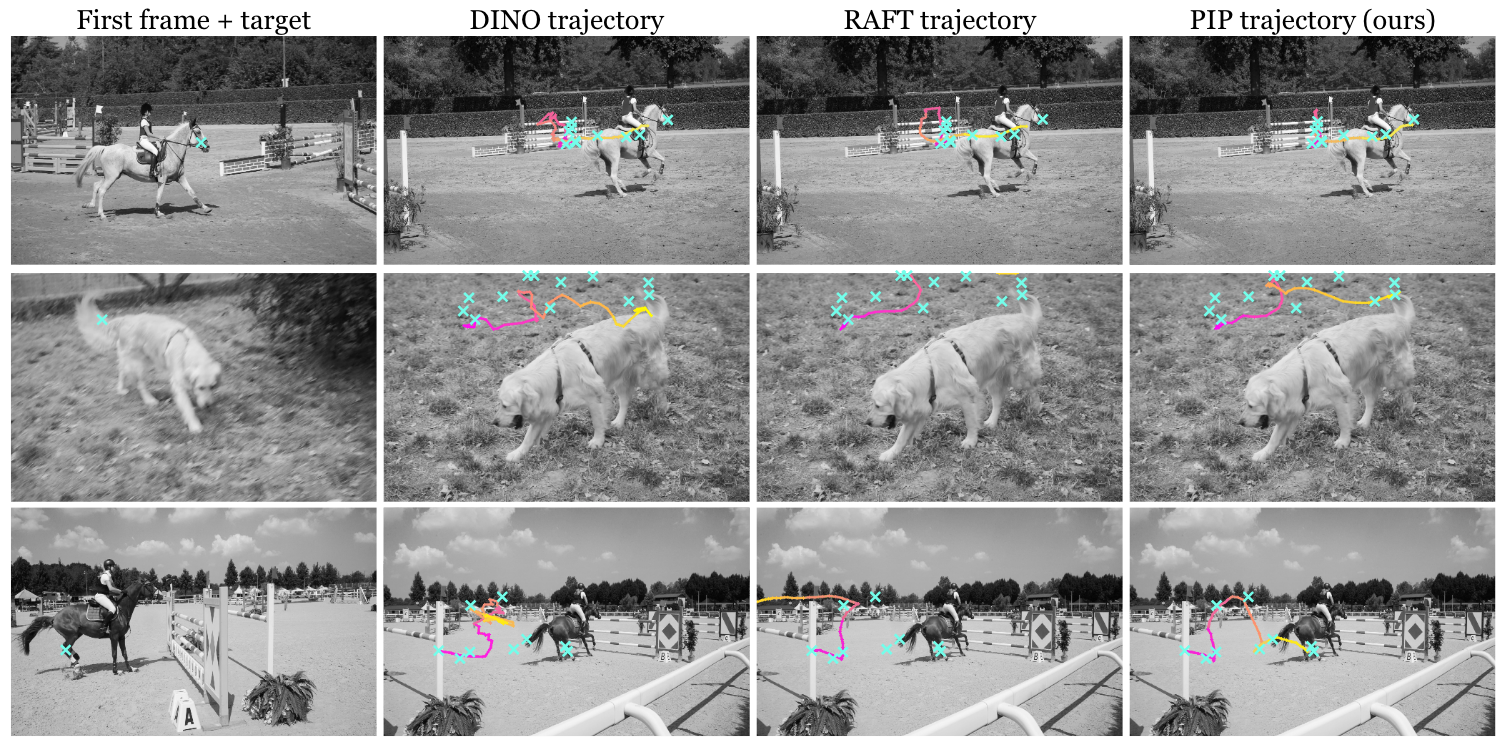
\includegraphics[width=0.85\linewidth]{images/PIPs_performance.png}    
    \caption{\textbf{Qualitative performance of PIPs on BADJA dataset against current state-of-art techniques.} Estimated trajectory of a tracked pixel is visualised by pink-to-yellow colourmap. Ground truth is represented by cyan × marks. We can see that PIPs successfully continues to track pixels that have been occluded, while other methods fail \citep{DBLP:journals/corr/abs-2204-04153}.}
    \label{fig:pips} 
\end{figure}

\section{Summary}
Summary here.
%==================================================================================================================================
\chapter{Analysis}
What is the problem that you want to solve, and how did you arrive at it?

\section{Guidance}
Make it clear how you derived the constrained form of your problem via a clear and logical process. 

%==================================================================================================================================
\chapter{Design} \label{design}
How is this problem to be approached, without reference to specific implementation details? 

\section{Guidance}
Design should cover the abstract design in such a way that someone else might be able to do what you did, but with a different language or library or tool.

%==================================================================================================================================
\chapter{Implementation} \label{implementation}
What did you do to implement this idea, and what technical achievements did you make?
\section{Guidance}
You can't talk about everything. Cover the high level first, then cover important, relevant or impressive details.



\section{General points}

These points apply to the whole dissertation, not just this chapter.



\subsection{Figures}
You may include multiple figures in one float, as in Figure \ref{fig:synthetic}, using \texttt{subcaption}, which is enabled in the template.



% \begin{figure}
%     \centering
%     \begin{subfigure}[b]{0.45\textwidth}
%         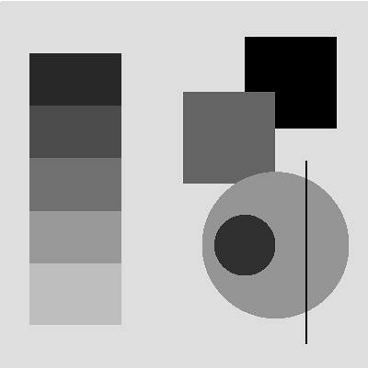
\includegraphics[width=\textwidth]{images/synthetic.png}
%         \caption{Synthetic image, black on white.}
%         \label{fig:syn1}
%     \end{subfigure}
%     ~ %add desired spacing between images, e. g. ~, \quad, \qquad, \hfill etc. 
%       %(or a blank line to force the subfigure onto a new line)
%     \begin{subfigure}[b]{0.45\textwidth}
%         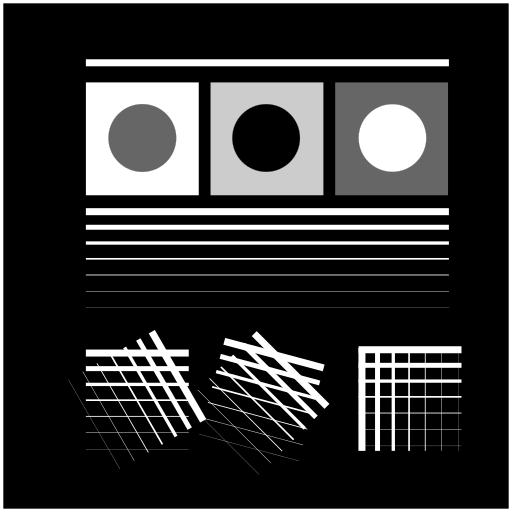
\includegraphics[width=\textwidth]{images/synthetic_2.png}
%         \caption{Synthetic image, white on black.}
%         \label{fig:syn2}
%     \end{subfigure}
%     ~ %add desired spacing between images, e. g. ~, \quad, \qquad, \hfill etc. 
%     %(or a blank line to force the subfigure onto a new line)    
%     \caption{Synthetic test images for edge detection algorithms. \subref{fig:syn1} shows various gray levels that require an adaptive algorithm. \subref{fig:syn2}
%     shows more challenging edge detection tests that have crossing lines. Fusing these into full segments typically requires algorithms like the Hough transform.
%     This is an example of using subfigures, with \texttt{subref}s in the caption.
%     }\label{fig:synthetic}
% \end{figure}

\clearpage

\subsection{Equations}

Equations should be typeset correctly and precisely. Make sure you get parenthesis sizing correct, and punctuate equations correctly 
(the comma is important and goes \textit{inside} the equation block). Explain any symbols used clearly if not defined earlier. 

For example, we might define:
\begin{equation}
    \hat{f}(\xi) = \frac{1}{2}\left[ \int_{-\infty}^{\infty} f(x) e^{2\pi i x \xi} \right],
\end{equation}    
where $\hat{f}(\xi)$ is the Fourier transform of the time domain signal $f(x)$.

\subsection{Algorithms}
Algorithms can be set using \texttt{algorithm2e}, as in Algorithm \ref{alg:metropolis}.

% NOTE: line ends are denoted by \; in algorithm2e
\begin{algorithm}
    \DontPrintSemicolon
    \KwData{$f_X(x)$, a probability density function returing the density at $x$.\; $\sigma$ a standard deviation specifying the spread of the proposal distribution.\;
    $x_0$, an initial starting condition.}
    \KwResult{$s=[x_1, x_2, \dots, x_n]$, $n$ samples approximately drawn from a distribution with PDF $f_X(x)$.}
    \Begin{
        $s \longleftarrow []$\;
        $p \longleftarrow f_X(x)$\;
        $i \longleftarrow 0$\;
        \While{$i < n$}
        {
            $x^\prime \longleftarrow \mathcal{N}(x, \sigma^2)$\;
            $p^\prime \longleftarrow f_X(x^\prime)$\;
            $a \longleftarrow \frac{p^\prime}{p}$\;
            $r \longleftarrow U(0,1)$\;
            \If{$r<a$}
            {
                $x \longleftarrow x^\prime$\;
                $p \longleftarrow f_X(x)$\;
                $i \longleftarrow i+1$\;
                append $x$ to $s$\;
            }
        }
    }
    
\caption{The Metropolis-Hastings MCMC algorithm for drawing samples from arbitrary probability distributions, 
specialised for normal proposal distributions $q(x^\prime|x) = \mathcal{N}(x, \sigma^2)$. The symmetry of the normal distribution means the acceptance rule takes the simplified form.}\label{alg:metropolis}
\end{algorithm}

\subsection{Tables}

If you need to include tables, like Table \ref{tab:operators}, use a tool like https://www.tablesgenerator.com/ to generate the table as it is
extremely tedious otherwise. 

\begin{table}[]
    \caption{The standard table of operators in Python, along with their functional equivalents from the \texttt{operator} package. Note that table
    captions go above the table, not below. Do not add additional rules/lines to tables. }\label{tab:operators}
    %\tt 
    \rowcolors{2}{}{gray!3}
    \begin{tabular}{@{}lll@{}}
    %\toprule
    \textbf{Operation}    & \textbf{Syntax}                & \textbf{Function}                            \\ %\midrule % optional rule for header
    Addition              & \texttt{a + b}                          & \texttt{add(a, b)}                                    \\
    Concatenation         & \texttt{seq1 + seq2}                    & \texttt{concat(seq1, seq2)}                           \\
    Containment Test      & \texttt{obj in seq}                     & \texttt{contains(seq, obj)}                           \\
    Division              & \texttt{a / b}                          & \texttt{div(a, b) }  \\
    Division              & \texttt{a / b}                          & \texttt{truediv(a, b) } \\
    Division              & \texttt{a // b}                         & \texttt{floordiv(a, b)}                               \\
    Bitwise And           & \texttt{a \& b}                         & \texttt{and\_(a, b)}                                  \\
    Bitwise Exclusive Or  & \texttt{a \textasciicircum b}           & \texttt{xor(a, b)}                                    \\
    Bitwise Inversion     & \texttt{$\sim$a}                        & \texttt{invert(a)}                                    \\
    Bitwise Or            & \texttt{a | b}                          & \texttt{or\_(a, b)}                                   \\
    Exponentiation        & \texttt{a ** b}                         & \texttt{pow(a, b)}                                    \\
    Identity              & \texttt{a is b}                         & \texttt{is\_(a, b)}                                   \\
    Identity              & \texttt{a is not b}                     & \texttt{is\_not(a, b)}                                \\
    Indexed Assignment    & \texttt{obj{[}k{]} = v}                 & \texttt{setitem(obj, k, v)}                           \\
    Indexed Deletion      & \texttt{del obj{[}k{]}}                 & \texttt{delitem(obj, k)}                              \\
    Indexing              & \texttt{obj{[}k{]}}                     & \texttt{getitem(obj, k)}                              \\
    Left Shift            & \texttt{a \textless{}\textless b}       & \texttt{lshift(a, b)}                                 \\
    Modulo                & \texttt{a \% b}                         & \texttt{mod(a, b)}                                    \\
    Multiplication        & \texttt{a * b}                          & \texttt{mul(a, b)}                                    \\
    Negation (Arithmetic) & \texttt{- a}                            & \texttt{neg(a)}                                       \\
    Negation (Logical)    & \texttt{not a}                          & \texttt{not\_(a)}                                     \\
    Positive              & \texttt{+ a}                            & \texttt{pos(a)}                                       \\
    Right Shift           & \texttt{a \textgreater{}\textgreater b} & \texttt{rshift(a, b)}                                 \\
    Sequence Repetition   & \texttt{seq * i}                        & \texttt{repeat(seq, i)}                               \\
    Slice Assignment      & \texttt{seq{[}i:j{]} = values}          & \texttt{setitem(seq, slice(i, j), values)}            \\
    Slice Deletion        & \texttt{del seq{[}i:j{]}}               & \texttt{delitem(seq, slice(i, j))}                    \\
    Slicing               & \texttt{seq{[}i:j{]}}                   & \texttt{getitem(seq, slice(i, j))}                    \\
    String Formatting     & \texttt{s \% obj}                       & \texttt{mod(s, obj)}                                  \\
    Subtraction           & \texttt{a - b}                          & \texttt{sub(a, b)}                                    \\
    Truth Test            & \texttt{obj}                            & \texttt{truth(obj)}                                   \\
    Ordering              & \texttt{a \textless b}                  & \texttt{lt(a, b)}                                     \\
    Ordering              & \texttt{a \textless{}= b}               & \texttt{le(a, b)}                                     \\
    % \bottomrule
    \end{tabular}
    \end{table}
\subsection{Code}

Avoid putting large blocks of code in the report (more than a page in one block, for example). Use syntax highlighting if possible, as in Listing \ref{lst:callahan}.

\begin{lstlisting}[language=python, float, caption={The algorithm for packing the $3\times 3$ outer-totalistic binary CA successor rule into a 
    $16\times 16\times 16\times 16$ 4 bit lookup table, running an equivalent, notionally 16-state $2\times 2$ CA.}, label=lst:callahan]
    def create_callahan_table(rule="b3s23"):
        """Generate the lookup table for the cells."""        
        s_table = np.zeros((16, 16, 16, 16), dtype=np.uint8)
        birth, survive = parse_rule(rule)

        # generate all 16 bit strings
        for iv in range(65536):
            bv = [(iv >> z) & 1 for z in range(16)]
            a, b, c, d, e, f, g, h, i, j, k, l, m, n, o, p = bv

            # compute next state of the inner 2x2
            nw = apply_rule(f, a, b, c, e, g, i, j, k)
            ne = apply_rule(g, b, c, d, f, h, j, k, l)
            sw = apply_rule(j, e, f, g, i, k, m, n, o)
            se = apply_rule(k, f, g, h, j, l, n, o, p)

            # compute the index of this 4x4
            nw_code = a | (b << 1) | (e << 2) | (f << 3)
            ne_code = c | (d << 1) | (g << 2) | (h << 3)
            sw_code = i | (j << 1) | (m << 2) | (n << 3)
            se_code = k | (l << 1) | (o << 2) | (p << 3)

            # compute the state for the 2x2
            next_code = nw | (ne << 1) | (sw << 2) | (se << 3)

            # get the 4x4 index, and write into the table
            s_table[nw_code, ne_code, sw_code, se_code] = next_code

        return s_table

\end{lstlisting}

%==================================================================================================================================
\chapter{Evaluation} \label{evaluation}
How good is your solution? How well did you solve the general problem, and what evidence do you have to support that?

\section{Guidance}
\begin{itemize}
    \item
        Ask specific questions that address the general problem.
    \item
        Answer them with precise evidence (graphs, numbers, statistical
        analysis, qualitative analysis).
    \item
        Be fair and be scientific.
    \item
        The key thing is to show that you know how to evaluate your work, not
        that your work is the most amazing product ever.
\end{itemize}

\section{Evidence}
Make sure you present your evidence well. Use appropriate visualisations, reporting techniques and statistical analysis, as appropriate.

If you visualise, follow the basic rules, as illustrated in Figure \ref{fig:boxplot}:
\begin{itemize}
\item Label everything correctly (axis, title, units).
\item Caption thoroughly.
\item Reference in text.
\item \textbf{Include appropriate display of uncertainty (e.g. error bars, Box plot)}
\item Minimize clutter.
\end{itemize}

See the file \texttt{guide\_to\_visualising.pdf} for further information and guidance.

\begin{figure}
    \centering
    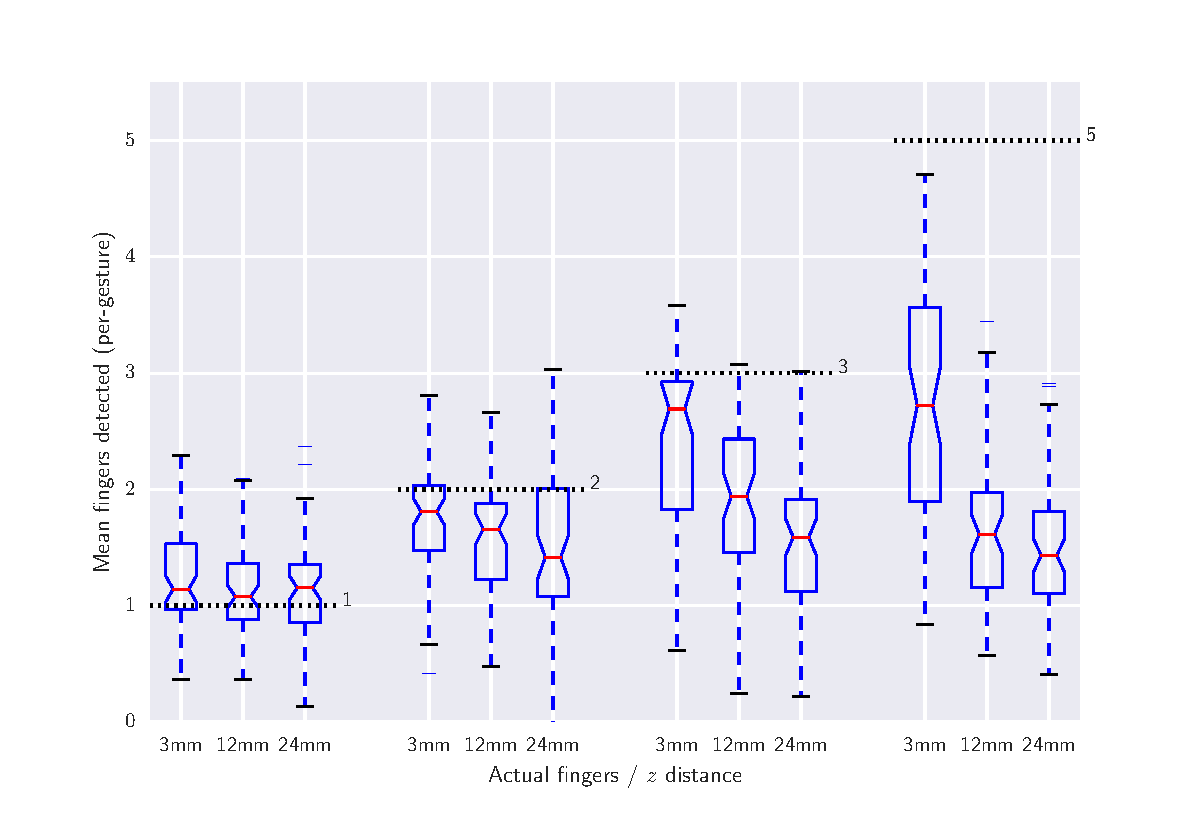
\includegraphics[width=1.0\linewidth]{images/boxplot_finger_distance.pdf}    

    \caption{Average number of fingers detected by the touch sensor at different heights above the surface, averaged over all gestures. Dashed lines indicate
    the true number of fingers present. The Box plots include bootstrapped uncertainty notches for the median. It is clear that the device is biased toward 
    undercounting fingers, particularly at higher $z$ distances.
    }

    % use the notation fig:name to cross reference a figure
    \label{fig:boxplot} 
\end{figure}


%==================================================================================================================================
\chapter{Conclusion}    
Summarise the whole project for a lazy reader who didn't read the rest (e.g. a prize-awarding committee).
\section{Guidance}
\begin{itemize}
    \item
        Summarise briefly and fairly.
    \item
        You should be addressing the general problem you introduced in the
        Introduction.        
    \item
        Include summary of concrete results (``the new compiler ran 2x
        faster'')
    \item
        Indicate what future work could be done, but remember: \textbf{you
        won't get credit for things you haven't done}.
\end{itemize}

%==================================================================================================================================
%
% 
%==================================================================================================================================
%  APPENDICES  

\begin{appendices}

\chapter{Appendices}

Typical inclusions in the appendices are:

\begin{itemize}
\item
  Copies of ethics approvals (required if obtained)
\item
  Copies of questionnaires etc. used to gather data from subjects.
\item
  Extensive tables or figures that are too bulky to fit in the main body of
  the report, particularly ones that are repetitive and summarised in the body.

\item Outline of the source code (e.g. directory structure), or other architecture documentation like class diagrams.

\item User manuals, and any guides to starting/running the software.

\end{itemize}

\textbf{Don't include your source code in the appendices}. It will be
submitted separately.

\end{appendices}

%=============================================================================================================================
%   BIBLIOGRAPHY   

% The bibliography style is abbrvnat
% The bibliography always appears last, after the appendices.

\bibliographystyle{abbrvnat}

\bibliography{l4proj}

\end{document}
